\section{Motivation}\label{sec:motivation}

\begin{figure}[tbp]
	\centering
	\subfloat[TODO: replace this image to avoid copyright problems.\label{fig:connected-vehicles}] {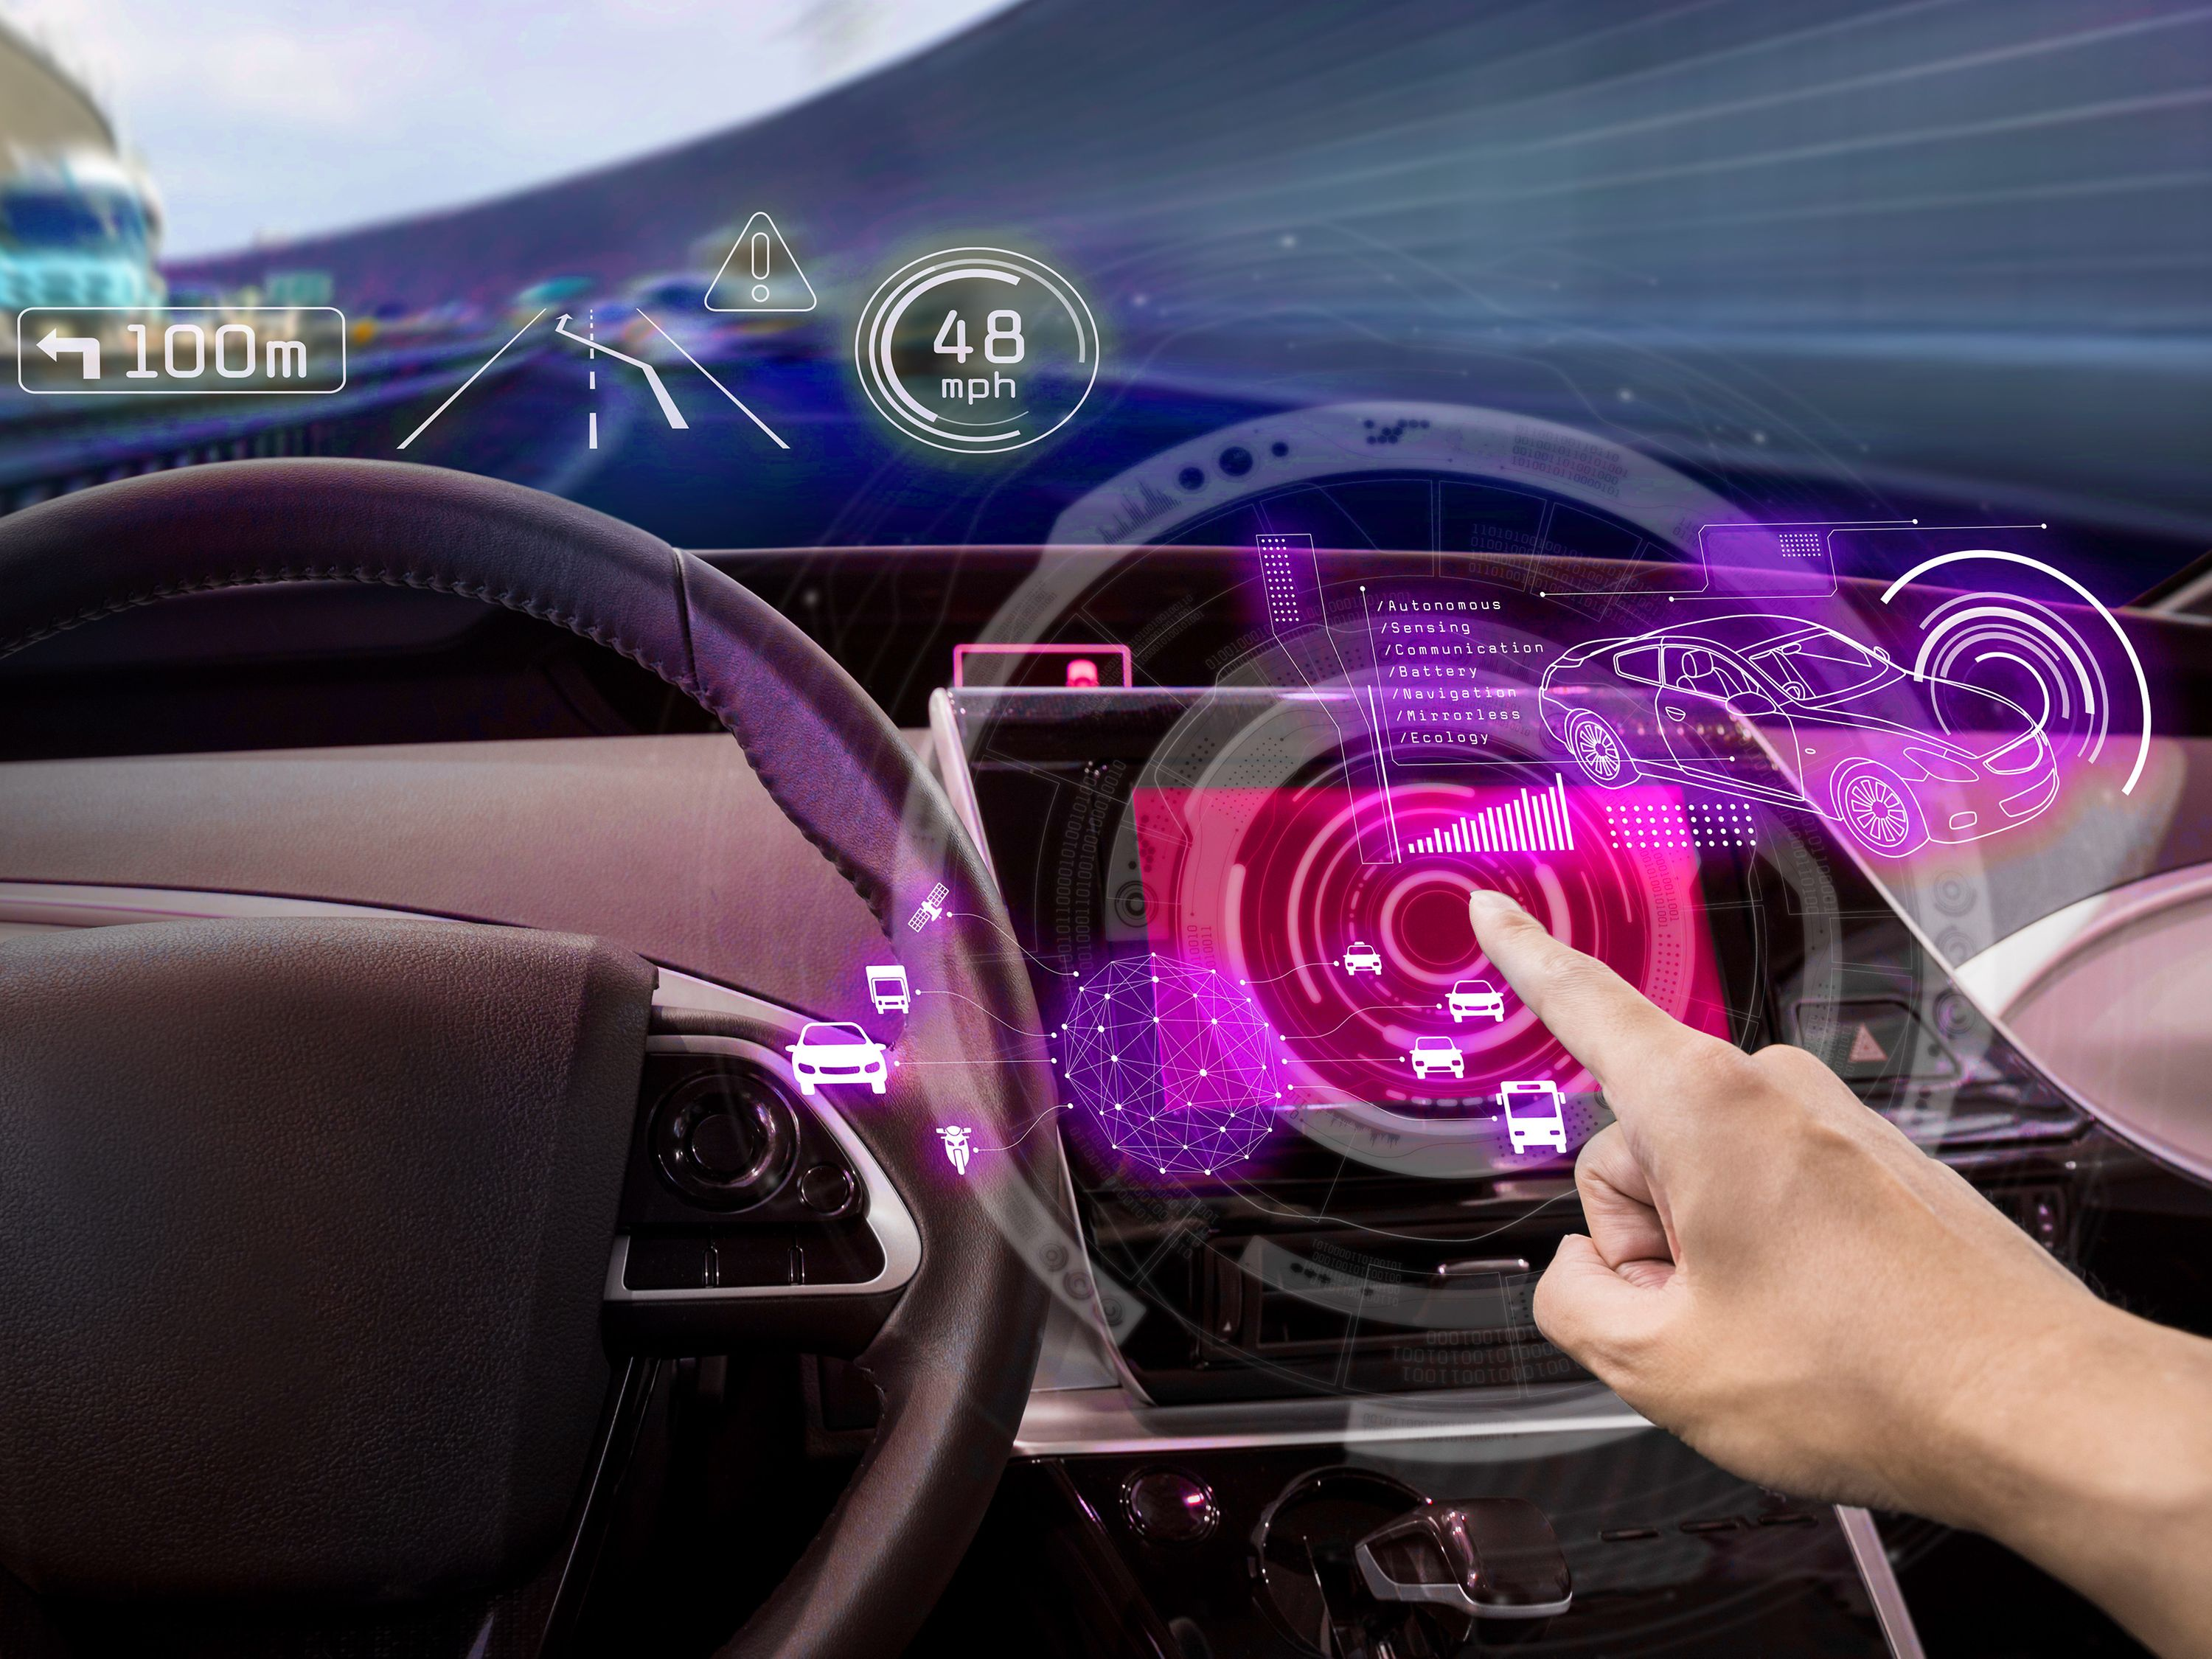
\includegraphics[width=0.47\textwidth]{figs/connected-vehicles.jpg}}\hfill
	~
	\subfloat[TODO: replace this with a less depressive image of augmented reality :)\label{fig:augmented-reality}]{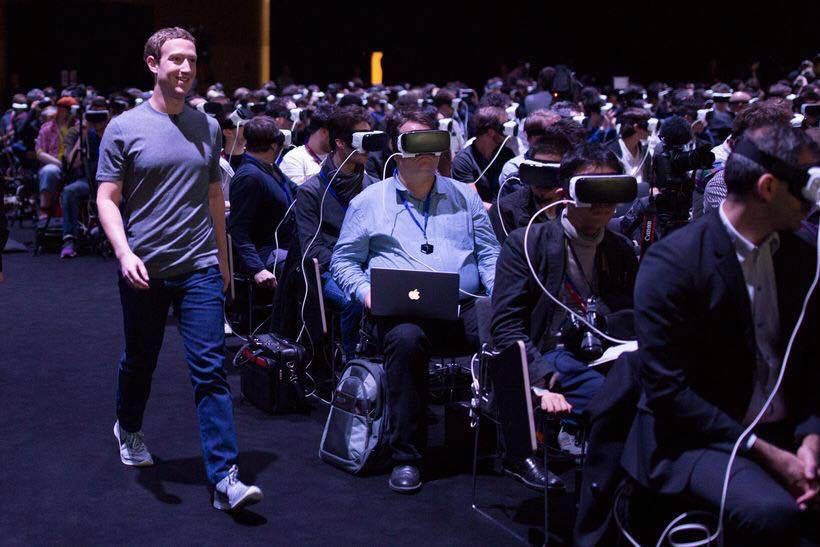
\includegraphics[width=0.53\textwidth]{figs/augmented-reality.jpg}}\hfill
	\caption{Different application types can be enabled or benefit from the low-latency of services deployed to nearby edge servers} \label{fig:motivational-cases}
\end{figure}

\subsection{Low-Latency Applications}

The main motivation for shifting computation from cloud to edge infrastructure is to mitigate network latency~\cite{Bonomi2014}. In specific, real-time applications are the main candidates for benefiting of services deployed at nearby edge infrastructure. Among these, some have a higher degree of criticallity with respect to latency and readiness of services (e.g., delay can have severe consequences to the users and/or the environment), whereas others can greatly benefit from lower latencies (e.g., by improving the user experience).

As an example of a critical application, connected vehicles (CV)~\cite{Bonomi:2012} are expected to be the computing device of the next decade, with each vehicle generating 25GB/hour of data~\cite{HitachiInternetOnWheels16}. In addition to local data analysis, more complex analysis shall be delegated to remote servers, which must respond quickly if the result involves critical information, e.g., the notification of an accident in the current path of the vehicle. With edge computing, computational resources located at mobile base stations or even composing the traffic infrastructure (e.g., highways) could provide low-latency services for connected vehicles passing by their coverage area.

Moreover, Augmented Reality (AR) is a type of application that would benefit from the low-latency of edge services~\cite{hu2015mobile,GarrigaMendonca2017}. These applications enrich the interaction of users with the physical
world by augmenting their vision of the reality with relevant information (e.g., historical information about buildings and monuments), modifying it (e.g., by translating captured text in a different language), or by adding virtual elements that can mimic interactions with the real world (e.g., virtual objects or creatures
from a fantasy game), or helping users fulfill physical tasks (e.g., by highlighting a free parking spot).

AR applications commonly depend on two key computational tasks: 1) extracting features from physical elements in the captured scene; and 2) matching these features against a feature database to obtain the corresponding information to be added to the scene. 

With the advent of mobile computing, AR applications can be deployed to companion devices like smartphones, tablets, and special purpose glasses. In many cases, these applications must process large volumes of data. Plus, this data can be volatile, which further limits the feasibility of storing it locally. Instead, data must be acquired from remote services. In order to augment the reality captured live from devices camera, the AR application needs to perform its tasks in a timely fashion, which poses a strong restriction on the latency requirement for remote services consumed. As such, a cloud-based solution tends to fail to meet this requirement~\cite{GarrigaMendonca2017}. 

%Additionally, image processing may over stress devices resources. This problem could be mitigated  
%architectural decision of where these tasks should be computed.

%AR applications that capture a live representation of the physical world, this reality must be augmented at real-time, meaning data must be retrieved in a timely fashion. Due to network latency, a cloud-based solution tends to fail. Accordingly, feature extraction task should be deployed near to client devices, e.g.., to edge servers. 

\begin{figure}[tbp]
	\centering
	\subfloat[Services are deployed to edge servers in order to reduce latency imposed by network communication with cloud servers \label{fig:cloud-to-edge}]{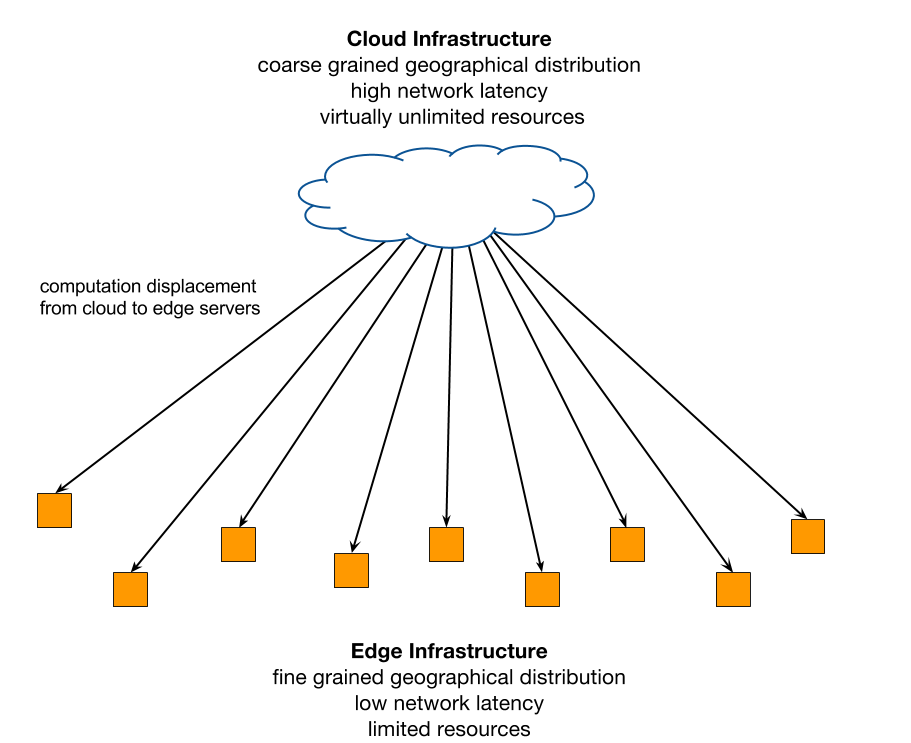
\includegraphics[width=0.45\textwidth,valign=t]{figs/cloud-to-edge.png}}\hfill
	~
	\subfloat[second caption.\label{fig:mobile-to-edge}] {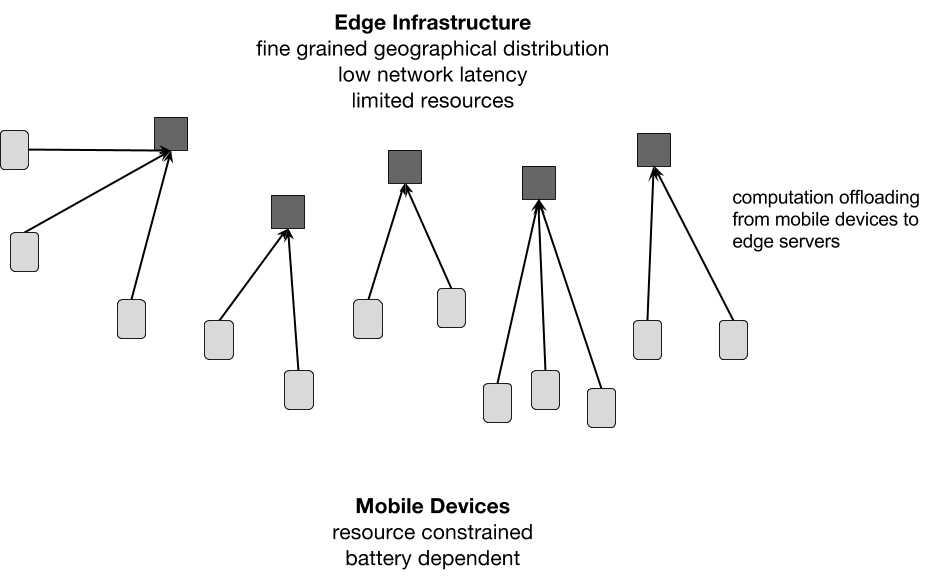
\includegraphics[width=0.55\textwidth,valign=t]{figs/mobile-to-edge.png}}\hfill
	\caption{General caption.} \label{fig:1}
\end{figure}

\subsection{Mobile Computation Offloading}

In addition to the problem of network latency, mobile devices exhibit limitations that may further motivate the use of edge computing. 

For instance, some mobile applications rely on heavyweight tasks that can overstress the platform and limit the concurrent execution of other applications. Moreover, battery is a valuable resource that may be significantly affected by the kind of computational task performed by mobile devices. 

In the paradigm of Mobile Cloud Computing (MCC)~\cite{Khan:14}, this problem has been addressed with the offloading of mobile computation to cloud servers. This approach, however, is limited by network latency. In contrast, edge computing could be an alternative to allow heavyweight or complex computation with low-latency requirements to be offloaded from resource constrained devices to nearby servers.

%The paradigm of edge computing can be explored to mitigate the problems related to the resource limitations of mobile devices. For this, heavyweight computation from mobile applications could be offloaded to nearby edge servers. 

As an example, the previously mentioned feature extraction task from AR applications is a type of heavyweight computation based on image processing. Instead of performing it locally (as proposed in~\cite{Huang2012}), mobile devices could also offload this task to nearby edge servers. 

\subsection{Computational Continuum}

\begin{figure}[tbp]
	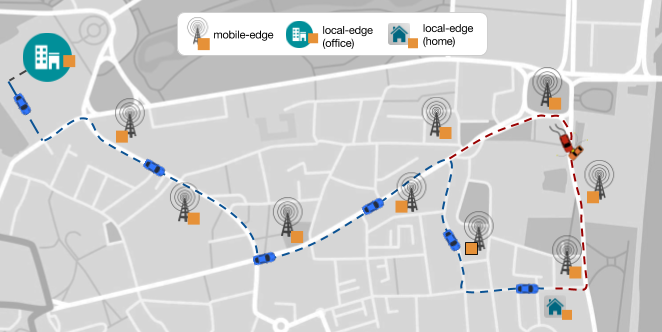
\includegraphics[width=0.9\textwidth]{figs/continuum.png}
	\caption{Heterogeneous applications (AR and CV) interact with services deployed along the computational continuum (cloud, mobile-edge, local-edge, and mobile)}
	\label{fig:continuum}
\end{figure}

Together, the computational resources from mobile, edge, and cloud computing have the potential of forming a \textit{computational continuum} on which new and disruptive types of applications can rely. 

To illustrate such scenario, we put together the two application examples previously described as part of a continuum that starts in the user's office and finishes in his home (Fig.~\ref{fig:continuum}). 

Let us assume the existence of a local edge server in the user's office (hereafter called \textit{local-edge}). This server is owned by the company to allow employees to extend the computational capabilities of mobile devices. The user, e.g., makes use of a \textit{smartglass} application to craft three dimensional virtual objects added to his desk table.

After work, our user leaves his office and enters his CV. During its way home, the autonomous vehicle will make use of edge services deployed at servers located at cellular base stations and owned by telecoms (hereafter called \textit{mobile-edge}). The connected vehicle gets low-latency updates about the best plan to reach its destination. For example, within milliseconds, the vehicle is suggested to make a turn just in time to avoid the traffic formed by an accident a few blocks ahead.

Already at home, the user's smartphone gets in reach of communication with the local-edge server owned by him. In that day, the user finds out about a new mobile game application that makes use of AR. Upon installation, the local-edge server becomes aware of a new edge-compliant application and meanwhile the user is already playing proceeds with the acquisition and deployment of the service into the local-edge server. After this, the client application becomes aware of these services and switches from local to edge with the purpose of preserving the smartphone's resources. Not only the game performance improves, but also the battery consumption is reduced.  

In the scenario described above, different parts of the continuum have been employed by user's devices. Whilst edge was privileged, cloud-based services remain fundamental, as edge infrastructure may not be available and services for which network latency is not disruptive are in the cloud (e.g., persistence, stateful components, and large part of the business logic).